\subsection{Konzept einer Wertschöpfungskette}\label{wsk}
Die in Abbildung \hyperref[img:supplychain]{7} dargestellte Supply Chain zeigt den Weg von der Entwicklung zum Absatz von Software an Kunden. Software Provider stellen Software für den Shop bereit und verdienen an einer verkauften Software. Sie können mit Service Providern zusammenarbeiten um so neue Funktionalitäten in Fahrzeugen zu schaffen und so zusätzlichen Umsatz generieren. Die im Software Store bereitgestellten Softwares können über das Internet heruntergeladen und im folgenden von Kunden genutzt und verwaltet werden.
\begin{figure}[!h]
	\centering
	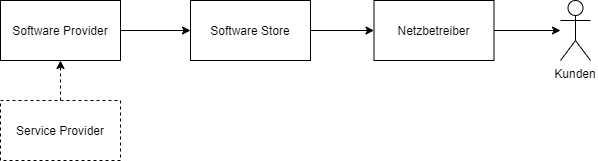
\includegraphics[width=0.8\columnwidth]{pictures/supplychain.png}
	\label{img:supplychain}
	\caption{Supply Chain von Software}
\end{figure}
Da die Erstellung eines Software Stores viele Aufgaben mit sich bringt, wird im folgenden ein Konzept einer Wertschöpfungskette für diesen erstellt. Diese soll die einen Überblick über die Aufgaben de Stores bieten.\\
Nach der Wertschöpfungskette von Porter sind Unternehmen in primäre und unterstützende Aktivitäten aufzuteilen.\footnote{quelle} Primäre Aktivitäten "liefern dabei einen direkten wertschöpfenden Beitrag zur Erstellung eines Produktes."\footnote{https://refa.de/service/refa-lexikon/wertschoepfungskette, 21. Mai 2020} Unterstützende Aktivitäten sind als "notwendige Voraussetzung zu Erstellung der Produkte"\footnote{ebd.} zu sehen, also Dinge die im Rahmen aller Primäraktivitäten wichtig sind. Abbildung \hyperref[img:wsk]{8} gibt einen Überblick der identifizierten Bausteine der einzelnen Aktivitäten, welche im folgenden genauer dargestellt werden. Im skizzierten Businessmodel wurde im Rahmen der Schlüsselaktivitäten bereits ein Unterteilung in unterschiedliche Aufgabenbereiche vorgenommen \textit{(Kap. \ref{key_activities})}, welche im folgenden für die Gruppierung der Bausteine verwendet wird.
\subsubsection{Primäre Aktivitäten}
Es gibt Fünf unterschiedliche Primäre Aktivitäten. Das Kaufen und Lagern von Materialien wird der \textbf{Eingangslogistik }zugeordnet. Im Kontext des Softwareshops gibt es hier Zwei wichtige Bausteine:
\begin{itemize}
	\item[] \hspace{-0.6cm}\textbf{Software-Sicherheit verifizieren}\\ \label{security}
	Sämtliche Softwares, die in dem Shop aufgeführt werden sollen, müssen durch ein Sicherheitskonzept verifiziert werden. Es sollten mehrere Sicherheitskonzepte und Richtlinien erarbeitet werden, auch zwecks einer Unterscheidung von Fahrfunktions- und Service Software. Diese Konzepte unterstützen die Bereitstellung von (sicherer) Software.\\
	Es muss sichergestellt werden, dass sämtliche erhobenen Daten entsprechend der Datenschutzrichtlinien des jeweiligen Landes verarbeitet werden. Neue Software muss außerdem auf Viren überprüft werden. Im Fall von \textit{Fahrfunktionssoftware }muss zudem sichergestellt werden, dass diese keine Sicherheitslücken in der Fahraufgabe aufweisen. Um dies zu erreichen, kann einer solchen Software eine Sammlung an OpenScenario Dateien beigefügt werden, die beschreiben welche Art von Situation durch die Software abgedeckt wird. Anhand dieser Dateien kann zum einen, wie in Kapitel \ref{2.2} beschrieben, die Suche von Softwares durchgeführt werden. Zum anderen können diese als Simulationsgrundlage dienen. Simulationen können Aussage darüber treffen, eine Software in der abzudeckenden Situation Sicher handelt oder nicht. Sie sollte auch im Rahmen der automatischen Erkennung von Softwarebedarf genutzt werden.
	
	\item[] \hspace{-0.6cm} \textbf{Klassifizierung von Software}\\
	Erfüllt eine Software die Sicherheitsrichtlinen, wird sie anschließend Klassifiziert. Eine Klassifizierung soll die entsprechenden Metadaten zu Softwares zuordnen, welche für die Einordnung im Shop notwendig sind. Dieser Schritt hat einen Direkten Bezug zur Bedarfserkennung von Software. Anhand der Klassifizierung sollen Fahrzeughalter intuitiv wissen, wie gut/schlecht eine Software ist und welche Aufgabe sie erfüllt. Hierzu muss ein Konzept erarbeitet werden, welches die Bewertungsfaktoren festlegt. In Kapitel \ref{sw_klassifizierung} wird eine Beispielkonzept vorgestellt.
\end{itemize}
\begin{figure}[!h]
	\hspace{-2.5cm}
	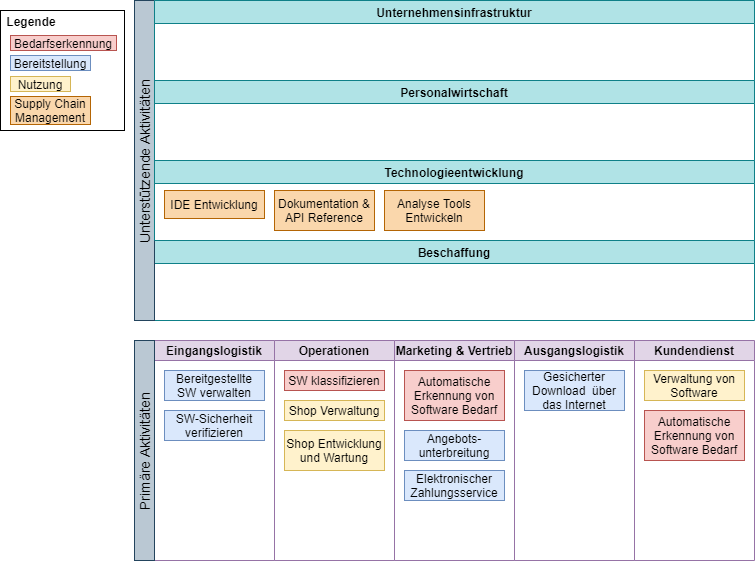
\includegraphics[width=1.2\columnwidth]{pictures/wsk.png}
	\label{img:wsk}
	\caption{Die wichtigsten Bausteine einzelner Aktivitäten der Wertschöpfungskette}
\end{figure}
Nach erfolgreichen Durchlaufen der Aktivitäten der Eingangslogistik folgen die Aktivitäten der \textbf{Operation}. Im Rahmen dieser werden die verifizierten und klassifizierten Softwares für den Absatz an Fahrzeughalter vorbereitet und auch absatz-unterstützende Aufgaben ausgeführt.
\begin{itemize}
	\item[] \hspace{-0.6cm} \textbf{Eigene Softwareentwicklung}\\
	Neben der Bereitstellung des Shops kann zusätzlicher Umsatz durch den verkauf eigener Software generiert werden. Hierdurch vergrößert sich nicht nur das Spektrum vorhandener Softwares, sondern es kann das allgemeine Image des Unternehmens positiv beeinflussen. Durch die innerbetriebliche Entwicklung kann auch der Verifikationsprozess der Software beschleunigt werden, was die Bereitstellung neuer Softwares ebenfalls früher ermöglicht.

	\item[] \hspace{-0.6cm}\textbf{Shop Verwaltung}\\
	Um die Kundenzufriedenheit weiter zu steigern, muss der Inhalt des Shops verwaltet werden. Einige Softwares sollen zeitweilig hervorgehoben werden, und auch die angezeigten 'vorgeschlagenen Softwares' müssen kontinuierlich an die Fahrzeugdaten angepasst werden.
	Softwares müssen hinzugefügt, entfernt oder aktualisiert werden und \textit{Empfehlungen der Redaktion} können gesetzt werden. Anstößige Kommentare oder gefährliche Softwares müssen aus dem Shop entfernt werden.\\
	Des weiteren muss gesteuert werden, welche Softwares den Fahrzeughaltern vorgeschlagen werden. Dies kann durch die Einbeziehung von Fahrdaten der Fahrzeugs geschehen, da so Softwares entlang der häufig zurückgelegten Strecken präsentiert werden könne,

	\item[] \hspace{-0.6cm} \textbf{Shop Entwicklung und Wartung}\\
	Auch die (Weiter-)Entwicklung und Wartung des Shops trägt zu einer höheren Kundenzufriedenheit bei. Änderungen im Frontend können die User Experience (UX) steigern und somit zum Kauf animieren. Bezüglich der Frontend Entwicklung sollten die Prinzipien des User Centered Designs beachtet werden. Änderungen des Backends können den Umfang des Shops erhöhen oder bisherige Funktionen \textit{(bspw. das Vorschlagen von Software)} verbessern und Kundenzentrierter gestalten.\\
	Für jegliche Änderungen sollte außerdem stets auf die Community gehört werden, welche sich aus den Software Providern und den Kundensegmenten zusammensetzt. Vorschläge und Wünsche für neue Softwares seitens der Kunden sollen evaluiert werden. Diese Vorschläge können möglicherweise veröffentlicht werden und von Providern  zur Ideenfindung genutzt werden. Die Zusammenarbeit mit Software Providern ist im Generellen sehr wichtig, weshalb im Rahmen der Unterstützenden Aktivitäten (\ref{unterstd_activities}) einige Bausteine zur Förderung dieser vorgestellt werden.	\\
\end{itemize}
Der Dritte Schritt einer Wertschöpfungskette ist zusammengesetzt aus dem\textbf{ Vermarkten des Software Shops und dem Vertrieb von Software. } Im Rahmen dieser finden sich die Bereitstellung unterstützende Bausteine in Form von Angebotsunterbreitung und der Bereitstellung einer elektronischen Zahlungsschnittstelle wieder. Außerdem findet hier die automatische, fahrzeug-individuelle Erkennung von Softwarebedarf statt.
\begin{itemize}
	\item[] \hspace{-0.6cm} \textbf{Automatische Erkennung von Software Bedarf}\\
	Um die Nutzenversprechen der \textit{automatischen Erkennung eines Software Bedarfs }zu erfüllen, müssen Serverseitige Algorithmen diese anhand von Fahrzeug und Fahrzeughalterdaten identifizieren. Hierfür ist eine Implementierung des Uptane-Standards \textit{(Kapitel \ref{3.1})} notwendig. \\
	
	Der Prozess automatischer Erkennung eines Software Bedarfs wird im folgenden skizziert. Zunächst muss hierfür das\textbf{ Manifest des Fahrzeugs zusammen mit Fahrdaten an den Server geschickt werden.} Im Manifest befindet sich eine Liste aller installierten Softwares des Fahrzeugs. Die verschickten Fahrdaten treffen Aussage darüber, welche Strecken vom Fahrzeug oft zurückgelegt werden. Auf dem Server angekommen, wird \textbf{entlang dieser Strecken nach möglichen Softwares für das Fahrzeug} gesucht. Wurden Softwares gefunden, die noch nicht auf dem Fahrzeug installiert sind werden mehrere \textbf{virtuelle Instanzen des Autos} erstellt. Eine dieser Instanzen umfasst nur die Softwares, welche laut dem Manifest auf dem fahrzeug installiert sind. Den anderen Instanzen wird jeweils eine Software hinzugefügt, die entlang der Strecken gefunden wurden.
	
	Nach dem erstellen dieser virtuellen Fahrzeuge werden im vierten Schritt die jeweiligen Situationen der neuen Softwares zugeordneten OpenScenario-Dateien \textbf{simuliert} und von den \textbf{virtuellen Fahrzeugen durchlaufen}. Zum Vergleich durchfährt das virtuelle Fahrzeug welches keine neuen Softwares erhalten hat die gleichen Situationen durch. Anhand eines Vergleichs der Simulationen kann festgestellt werden, ob die Software positive, negative oder überhaupt keine Auswirkungen auf das Fahrverhalten des Fahrzeugs hat. Positiv wäre, wenn das Fahrzeug die Situation nun selbstständig durchfahren kann oder dies Ressourcenschonender tut. Negativ wäre, wenn die Situation durch die neue Software nicht weiter durchfahren wird oder die neue Software zum durchfahren der Situation nicht vom Fahrzeug ausgewählt wird. Dies kann bedeuten, dass auf dem Fahrzeug bereits eine Software installiert ist, welche diese bereits abdeckt.\\
	
	Abhängig davon wie neue Softwares bei diesen Simulationen abschneiden werden sie anschließend dem Fahrzeughalter vorgeschlagen oder auch nicht. Durch diesen Prozess wird nicht nur die Kundenzufriedenheit gesteigert, sondern auch mehrere Nutzenversprechen  erfüllt bzw. erarbeitet \textit{(NV-3, NV-4, NV-5)}.
	
	Die in Kapitel \ref{2.3} vorgestellte Möglichkeit der direkten Suche anhand einer Situation sollte im übrigen auch bedacht werden. Sie kann ebenfalls automatisiert werden, indem das Fahrzeug automatische Suchanfragen an den Server verschickt, sobald eine nicht bewältigbare Situation auftritt.
	
	\item[] \hspace{-0.6cm} \textbf{Angebots Unterbreitung}\\
	Die Angebots Unterbreitung hat Zwei wichtige Bestandteile: Zum einen die Erstellung eines Angebots unter Beachtung der in Kapitel \ref{angebotserstellung} dargestellten Prinzipien. Zum anderen ist der Zeitpunkt, zu dem die Software dem Fahrer vorgeschlagen wird geeignet gewählt sein. Hierfür kann der in Kapitel \ref{3.3} vorgestellte SUPR implementiert werden. Die Fahrzeughalter sollen die Kaufart \textit{(i.e. Kauf, Miete, Abo)} selber auswählen können und so das Angebot zugunsten ihrer Zwecke abändern.
	
	\item[] \hspace{-0.6cm} \textbf{Bereitstellung elektronischer Zahlungsschnittstellen}\\
	Damit der Kauf von Fahrzeughaltern getätigt werden kann, muss mindestens eine gängige Zahlungsschnittstelle \textit{(MasterCard\footnote{}, PayPal\footnote{}, o.A.)} zur Verfügung gestellt werden. Durch multiple Zahlungsschnittstellen kann ein größerer Kundenstamm erreicht werden. Um weitere eigene Umsätze zu generieren, kann hier auch eine eigene Schnittstelle eingefügt werden. Hierdurch kann ein weiterer Betriebszweig \textit{(Bank)} aufgebaut werden. Fahrzeughalter können zum Nutzen dieser gebracht werden, indem der Kauf mittels dieser Schnittstelle beispielsweise günstiger ist. Ohne eine elektronische Zahlungsschnittstelle ist das betrieben des Shops und somit die orts- und zeitunabhängige Bereitstellung von Software nicht möglich.
	
	\item[] \hspace{-0.6cm} \textbf{Marketing}\\
	Wie im Business Model beschrieben, ist der Umfang des Marketings maßgebend für den Erfolg des Shops. Das Marketingkonzept sollte auf möglichst vielen Kanälen zu sehen sein und dabei möglichst viele Alters- und Kundengruppen ansprechen. Es können Studien herangezogen werden, wie der Google Playstore oder andere vergleichbare Plattformen sich entwickelt haben. Außerdem ist es ratsam "Markenbotschafter" zu finden, die Content für Social Media Plattformen entwerfen. Coca Cola hat dies beispielsweise erfolgreich mit Coke TV\footnote{text} geschafft.
\end{itemize}
Im Anschluss an das Vermarkten und Vertreiben von Software muss diese auch "ausgeliefert" werden. Die in diesem Aspekt anfallenden Bausteine werden dem Vierten Schritt einer Wertschöpfungskette, der \textbf{Ausgangslogistik} zugeordnet.
\begin{itemize}
	\item[] \hspace{-0.6cm} \textbf{Gesicherter Download über das Internet	}\\
	Die Bereitstellung von Software wird mit dem Download abgeschlossen. Dieser Download soll zum einen orts- und zeitunabhängig sein, außerdem muss die Download Schnittstelle sicher sein. Um ersteres zu gewährleisten, sollte der 5G-Ausbau zusammen mit den Mobilfunkanbietern und anderen gefördert werden. Außerdem ist eine Kooperation mit Mobilfunkanbietern denkbar, da eine Vielzahl von Autos künftig große Mengen an Daten verschicken werden. Dadurch könnten für die Fahrzeughalter oder auch für Shopbetreiber immense Kosten entstehen. Durch eine Partnerschaft können die Kosten skalierbar gehalten werden, indem Mobilfunkanbieter, Shopbetreiber und Automobilhersteller zugunsten der Kundenzufriedenheit kooperieren.
\end{itemize}
Damit die langfristige Zufriedenheit von Kunden sichergestellt werden kann, müssen auch nach dem Kauf für den Kunden wertschöpfende Aktivitäten durchgeführt werden. Diese werden dem letzten Schritt der Wertschöpfungskette, dem \textbf{Kundendienst}, zugeordnet.	
\begin{itemize}
	\item[] \hspace{-0.6cm} \textbf{Verwaltung von gekaufter Software}\\
	Damit Fahrzeughalter wissen, welche Softwares sie gekauft, geliehen oder gemietet haben soll für sie die eigenständige Verwaltung von Software möglich sein. Softwares sollen auch "deaktiviert" werden. Hierdurch behalten Fahrzeughalter im übrigen auch den Überblick.
	
	\item[] \hspace{-0.6cm} \textbf{Überwachung installierter Software}\\
	Um Fahrzeughaltern vor Augen zu führen, welche Softwares nötig für das Fahrzeug sind und welche nicht, sollten diese Einblick in eine Art Überwachung der Software erhalten. Hier können Grundlegende Statistiken geführt werden wie
	\begin{itemize}
		\item die durchschnittliche Nutzungsdauer der Software in Prozent
		\item das Datum, an welchem die Software das letzte mal genutzt wurde
		\item oder eine Liste, in welcher zu sehen ist welche Softwares an welchem Tag der Woche vermehrt genutzt werden.
	\end{itemize}
	Aufgrund der steigenden Bedeutung des Datenschutzes könnte auch eine Ansicht ertsellt werden, welche zeigt welche Daten von Softwares erhoben werden. Hierdurch könnte das Vertrauen von Kunden gestärkt werden \textit{(Oder auch nicht, je nach dem welche und wie viele Daten erhoben und gespeichert werden)}.
	
	\item[] \hspace{-0.6cm} \textbf{Kundenservice und Beratung}\\
	Um vor allem die Bindung zu älteren Kunden aufzubauen, kann das einrichten einer Telefonischen Beratung für große Softwarekäufe gut sein. Bei der Ersteinrichtung eines Fahrzeugs können Fahrzeughalter hierdurch unterstützt werden. Auch ein klassischer Kundenservice kann gut sein. Dieser Kundenservice muss nicht telefonisch erfolgen, sondern reicht auch in Form von Kommentare, Bewertungen und Feedback im Hinblick einer Software oder des Shops im generellen.
\end{itemize}
\textbf{Überblick}\\
Wird Software von Software Providern beim Softwareshop eingereicht, durchläuft sie die Fünf Schritte der Wertschöpfungskette. Jeder einzelne trägt dazu bei, das Fahrzeughalter am ende selbstständig genau die Software installieren können, die sie benötigen.
\begin{itemize}
	\item[1.] \textbf{Eingangslogistik}\\
	Anfangs muss die Sicherheit von Software verifiziert werden und es müssen Metadaten und Kennwerte für die Software festgelegt werden. Beides unterstützt die Nutzung des Shops.
	\item[2.] \textbf{Operationen}\\
	Ist die Software bereit für die Aufnahme in den Shop, muss sie dort eingepflegt werden. Innerbetrieblich hergestellte Software wird ebenfalls dem Shop hinzugefügt. Dieser wird immer weiterentwickelt und passt sich den Anforderungen der Nutzer an. 
	\item[3.] \textbf{Marketing und Vertrieb}\\
	Der Vertrieb von Software wird durch die automatische Erkennung eines Softwarebedarfs gekennzeichnet. Kunden kriegen Vorschläge, die auf der Basis ihrer eigenen Fakten und Statistiken beruhen. Das unterbreiten eines elektronisch abschließbaren Angebots lässt die Fahrzeughalter Softwares kaufen.
	\item[4.] \textbf{Ausgangslogistik}\\
	Bei der Verteilung der Software muss ein sicherer Download möglich sein. Hierzu ist es notwendig, in den Ausbau von Netzwerkstrukturen zu investieren.\footnote{Quelle}
	\item[5.] \textbf{Kundendienst}\\
	Zur Steigerung der Kundentreue und -zufriedenheit ist das bereitstellen einer vielzahl von Kundendiensten notwendig. Diese ermöglichen unter anderem das Verwalten und Überwachen installierter Softwares.
\end{itemize}
Während all diese Schritte durchlaufen werden, geben die \textit{unterstützenden Aktivitäten} stetig Mehrwerte zur Produktion hinzu. Sie sind also \textit{indirekt am Erfolg beteiligt.} Diese werden im folgenden vorgestellt und ihre Rolle im Ablauf der Wertschöpfungskette verdeutlicht.
\subsubsection{Unterstützende Aktivitäten}\label{unterstd_activities}
Es gibt Vier Unterstützende Aktivitäten. So ist eine sinnvolle \textbf{Unternehmensinfrastruktur} zu schaffen, mit guter Anbindung zur Außenwelt, schnellem Internet und Mitarbeiter freundlichen Büroräumen, in welchen auch Freizeitaktivitäten möglich sind. Weiterhin gibt es auch die \textbf{Personalwirtschaft}, oder auch Humnan-Resource-Management. Diese beschreiben wichtige, die Mitarbeiter unterstützende Strukturen und Anhaltspunkte.
\begin{itemize}
	\item[] \hspace{-0.6cm} \textbf{Weiterbildungen}\\
	Die kontinuierliche Weiterbildung der Entwickler, so zum Beispiel das gemeinsame lernen neuer Programmiersprachen \& -frameworks, oder auch gemeinsame Entwicklung des eigenen Lifestyles. Weiterbildungen können \textbf{alles} sein, was die Mitarbeiter voran bringt. Nicht nur Aspekte des Arbeitsgebiets sondern auch persönliche Skills tragen maßgebend dazu bei, dass Mitarbeiter aufgrund höherer Zufriedenheit besser arbeiten.\footnote{quelle} Das gemeinsame Lernen einer neuen Programmiersprache für die Back-End Entwicklung unterstützt direkt die (Weiter-)Entwicklung des Shops, welche im Kontext der Operationen durchgeführt wird.
\end{itemize}
Im Kontext eines Software Shops ist die stetige \textbf{Technologieentwicklung} wegweisend für den Erfolg des Unternehmens.\footnote{quelle} Hierzu gehört nicht nur die Schaffung von Werten für die innerbetriebliche Wertschöpfungskette, sondern auch die Supply Chain übergreifend Unterstützung der Partner und Kunden.

\begin{itemize}
	\item[] \hspace{-0.6cm} \textbf{IDE Entwicklung}\\
	Das entwickeln einer eigenen Entwicklungsumgebung\textit{(IDE)} für die Entwicklung von Software kann sowohl die eigene Softwareentwicklung als auch die anderer Software provider unterstützen. Mit designierten Simulatoren und integrierten Sicherheitschecks könnte der Weg von Idee über Entwicklung hinzu Bereitstellung im Shop verkürzt werden. Diese sollte immer weiterentwickelt werden und neue Funktionen erhalten, die den Entwicklungsvorgang unterstützen oder sogar beschleunigen. Ein Vergleich aus der Realität ist hier Android Studio aber auch die Eclipse IDE, welche in Zusammenarbeit mit Unternehmen aus der ganzen Welt entwickelt wird.
	
	\item[] \hspace{-0.6cm} \textbf{Dokumentation und API-Reference}\\
	Die Entwicklung von Software wird zusätzlich von der Bereitstellung einer ausführlichen API-Reference und einer technischen Dokumentation (mit Beispielen) positiv unterstützt. Die API-Reference sollte alle Funktionen von Klassen ausführlich beschreiben und im Nutzungskontext vorstellen. Diagramme unterstützen zusätzlich das Verständnis der API. Eine technische Dokumentation kann sehr vielfältig sein. Um die Entwicklung neuer Softwares voranzutreiben ist es Sinnvoll eine Einführung \textit{('Getting Started Guide')} in die Entwicklung von Softwares für ein Fahrzeug zu geben. Google stellt in diesem Kontext das \textit{Android Jetpack}\footnote{https://developer.android.com/jetpack} sowie weitere Dokumentationen mit Anleitungen und Videos zur Verfügung.\footnote{https://developer.android.com/guide}. Auch und vor allem sollten hier die Sicherheitskriterien welche im Kontext der Wertschöpfungskette in Abschnitt \ref{security} erwähnt wurden vorgestellt werden. Tipps und Tricks und zu beachtende Dinge sollten hier zu finden sein.
	
	\item[] \hspace{-0.6cm} \textbf{Entwicklung von Analyse-Tools}\\
	Um Statistiken bzgl. der Softwarenutzung überblicken zu können, sollten Analyse-Tools entwickelt werden. Dank einer Web-App, über welche Software Provider generelle\textit{(Nutzung in H je Tag)} und auch spezifischere\textit{(Button-Clicks)} Statistiken ihrer Softwares sehen können, wären Entwickler dazu in der Lage ihre Software zu verbessern.
	
	\item[] \hspace{-0.6cm} \textbf{API-Entwicklung}\\
	Neben einer ausführlichen API-Reference, muss die API selber stets erweitert werden. Hier gibt es zum einen die Software-API. Über diese müssen Systeme des Fahrzeugs angesteuert werden können und im generellen auch festgelegt werden wie die Software angesteuert wird. Die Weiterentwicklung der Software-API kann das ansteuern neuer Automarken oder die Anbindung an eine neue Schnittstelle umfassen. 
\end{itemize}
Die letzte unterstützende Aktivität ist die \textbf{Beschaffung}. Ihre Aufgabe ist, dass alle Mitarbeiter mit den nötigen Materialien, das heißt Computern, Tastaturen, Stiften oder anderem versorgt werden.\\\\